\chapter{Methods and materials.}

For this work, many diferent tools were used, which will be cathegorized in hardware, software and mathematical tools. \\

In terms of hardware, the author was granted access to the \textit{FQM-378} clusters in the Universidad de Córdoba. Access to these clusters was crucial for the calculations done throughout the work, reducing the time needed for each calculation in several orders of magnitude. Besides the clusters, the author also needed his own personal computer, mainly to remotely access the clusters and also for other types of calculations that could not have been done from the clusters. These calculations include among other things, plotting of figures.  \\

The main mathematical tool for this work was the Fourier Transform. The Fourier Transform is a consequence of Fourier's Theorem. This theorem states that for every `nice'\footnote{The conditions for which this theorem does not apply are beyond the scope of this work, and so the `niceness' of a function need not be defined} periodic function $f(x)$ of period $L$ one can find a unique linear combination of sine and cosine functions such that 
\begin{align}
	f(x) = C + \sum_\text{n odd} a_n \sin\left( \frac{nx}{L} \right) + \sum_{\text{n even}}^{} b_n \cos \left( \frac{nx}{L} \right) 
\end{align}
With $C $, $a_n$, $b_n$ given by\footnote{The subscript in $\int_{L}^{} $ only implies the integration over the length $L$, since it can be proven that any periodic function $f(x)$ with period L verifies $ \int_{0}^{L} f(x)dx = \int_{a}^{L+a} f(x)dx $ for any value of $a$. This is, the point at which the integral begins makes no difference, as long as the integration is done over a whole period. }
\begin{align}
	\begin{cases}
		C &= \frac{1}{L} \int_{L}^{} f(x) dx\\
		a_n &= \frac{1}{L} \int_{L}^{} f(x) \sin\left(  2\pi \frac{nx}{L} \right) dx,~\text{n odd}\\
		b_n &= \frac{1}{L} \int_{L}^{} f(x) \cos\left(  2\pi \frac{nx}{L} \right) dx,~\text{n even}\\
	\end{cases}
\end{align}\\

This was the original Fourier's result. However this theorem can be expanded to the complex realm as 
\begin{align}
	f(x) = \sum_{n=0}^{\infty} c_n e^{i 2\pi \frac{nx}{L}}, \text{with } c_n = \frac{1}{L}\int_{L}^{} f(x) e^{-i 2\pi \frac{nx}{L}}dx 
\end{align}
For each mode $n$ one can define a new variable $k=2\pi n /L$, leading to the actual definition of the Fourier Transform 
\begin{align}
	\tilde{f}(k) = \frac{1}{2\pi}\int_{L}^{}  f(x) e^{-i k x} dx
\end{align}
In this work, the power spectrum $P(k)$ is considered, which is the Fourier Transform of the correlation function $\xi(r)$.  Recalling the definition of the $\xi(r)$ function, the frequency of the distance at which two any two galaxies are found, one can notice that  $\xi(r)$ must be a discrete function. We thus define the Discrete Fourier Transform (DFT) over a discrete set of N data points $\{\left( x_i, \xi(x_i) \right) \}_{i=1}^{N} $
\begin{align}
	P(k_j) = \frac{1}{2\pi}\sum_{i=1}^{N} e^{-i k_j x_{i}} \xi(x_i)
	\label{eq:DFT}
\end{align}
Though one must think that the periodic function hypothesis is being broken, since of course the universe is not made of repeating blocks of the galaxies that surround us. That the universe is infinitely big and repeating is an assumption that needs to be done in order to calculate this Fourier Transform. In other words, these calculations asume periodic boundary conditions.\\


Another thing to be noted is the fast growing complexity of the algorithm described by \eqref{eq:DFT}, which grows as $N^2$, with $N$ the number of points used for the calculation. 
To solve this one would use the Fast Fourier Transform (FFT), instead of the DFT. This algorithm is based in the decomposition of the space considered with $N=N_1N_2$ data points, into two smaller spaces with $N_1$ and $N_2$ data points. It then factorizes each problem into smaller problems, and recursively breaks the configuration down into even smaller problems, thus greatly reducing the complexity of the algorithm from $N^2$ to $N\log N$. \\

The $P(k)$ has been until now only been vaguely defined. Let  $\rho(\textbf{x})$ determine the density of galaxies at a given point and $ \overline{\rho}$ the average density throughout the universe. As the interest lays in the fluctuations around the density, it is only natural to be interested in the overdensity $\delta(\textbf{x})$ at some position $\textbf{x}$
\begin{align}
	\delta(\textbf{x}) = \frac{\rho\left( \textbf{x} \right) - \overline{\rho}}{\overline{\rho}}
	\label{eq:overdensity)}
\end{align}
From this magnitude one calculates the aforementioned correlation function $\xi(\textbf{r})$ as\footnote{Note only the dependency on $r = \|\textbf{r}\|$ remains, since the universe is (assumed to be) homogenous and isotropic}
\begin{align}
	\xi(\textbf{r}) = \left<\delta(\textbf{x}) \delta(\textbf{x}') \right> = \frac{1}{V}\int_{V}^{}  d^3 \textbf{x} \delta(\textbf{x}) \delta\left(\textbf{x} - \textbf{r}  \right) 
\end{align} with $\textbf{r} = \textbf{x} - \textbf{x}'$
And the power spectrum is then defined as its three dimensional Fourier Transform.\\

To calculate $P(k)$ one then needs three coordinates for each galaxy (as would be expected from a three dimensional universe). These coordinates will be 2 angular coordinates (the declination $\delta$ and right ascension $\alpha$) and a radial coordinate $r$ which must be calculated from $z$. For this it is necessary to assume a cosmology, since it is what dictates the conversion from redshift to distance through Hubble's law \eqref{eq:ley-hubble}. For this transformation, the redshift is interpreted as a Doppler shift. At low enough velocities, $z\approx v /c$ and so \eqref{eq:ley-hubble} can be approximated to 
\begin{align}
c z = H_0 r	
\end{align}\\

The last step to calculate the power spectrum is to interpolate in between each galaxy, similar to how one would build a heatmap. This way the catalogue is continuous and no longer discrete. Now, with a continuous density function $\rho(\textbf{x})$ all necessities for the power spectrum are met and it can be finally calculated.\\

All these magnitudes are related to what is called the second moment of the overdensity. In general, the $n$th moment $\mu_n$ of some magnitude $x$ with a probability distribution $P(x)$ is defined as 
\begin{align}
	\mu_n = \int_{-\infty}^{\infty} x^{n}P(x)dx 
	\label{eq:n-moment}
\end{align}
It is then natural to ask why is only the second moment of the overdensity $\delta$ considered.\footnote{The dependency on $\textbf{x}$ was dropped since $\delta$ can be both spoken of in configuration space and momentum (Fourier) space. These representations correspond to the $\xi(r)$ and $P(k)$ functions, respectively.}
It has been measured in the CMB that the universe is a gaussian field. These kinds of fields have the property that any moment $\mu_n$ with $n>2$ will be 0. These moments (e.g. $ \left<\delta(\textbf{x}) \delta(\textbf{y}) \delta(\textbf{z}) \right>$) have been shown to all be compatible with 0. This is predicted by the inflation theory, but the strongest reason to believe this is the experimental data.\\

All these calculations are performed by Rapid foUrier STatIstics COde (RUSTICO)\cite{rustico}. This software needs the specific galaxy catalogue to be used, and the statement of the cosmology that is going to be used, in a similar fashion as was done in~\ref{sec:LCDM}. The catalogue to be used in this work is the Luminous Red Galaxy sample from the extended Baryon Oscillation Spectroscopic Survey (LRG eBOSS~\cite{eBoss}).
With this information it then takes the mentioned steps: Transforms each redshift $z$ to a radial distance $r$, assigns each galaxy to a point $\textbf{x}$, calculates through interpolation the galaxy density at each point $\rho\left(  \textbf{x}\right)$, the overdensity at each point $\delta\left( \textbf{x} \right)$, the correlation function $\xi(r)$ and finally its FFT to obtain the power spectrum $P(k)$, as seen in the figure~\ref{fig:rustico}. \\\\


\begin{figure}[t]
	\centering
	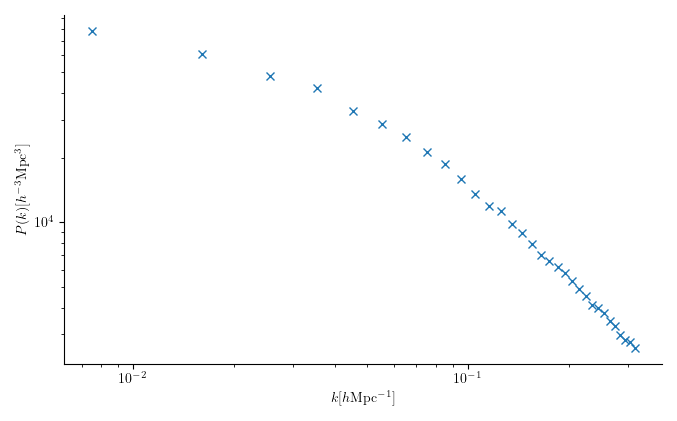
\includegraphics[width=0.8\textwidth]{../figs/Pkrustico.png}
	\caption{The power spectrum $P(k)$ of the LRG eBOSS~\cite{eBoss} catalogue as calculated by RUSTICO ($\Omega_k = 0.00$)}
	\label{fig:rustico}
\end{figure}

\begin{figure}[t]
	\centering
	\subfigure{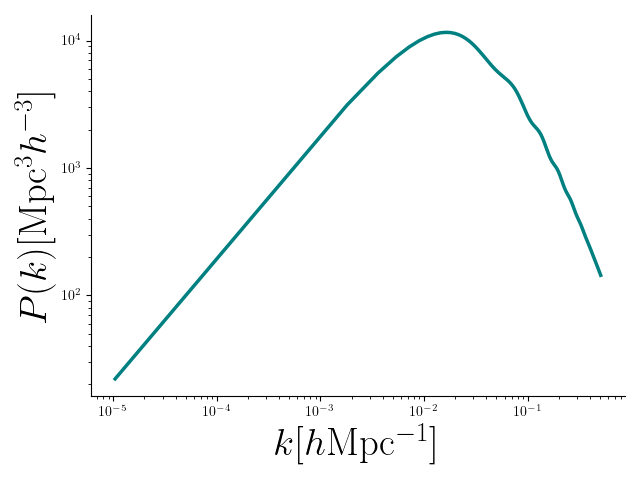
\includegraphics[width=0.3\textwidth]{../figs/Pklin.png}}
	\subfigure{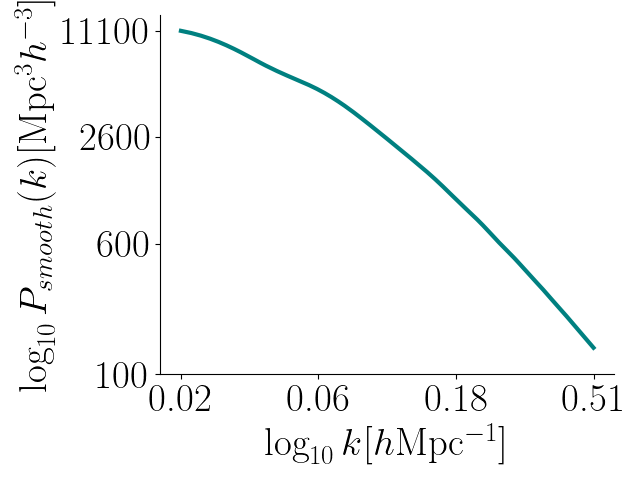
\includegraphics[width=0.3\textwidth]{../figs/Psm.png}}
	\subfigure{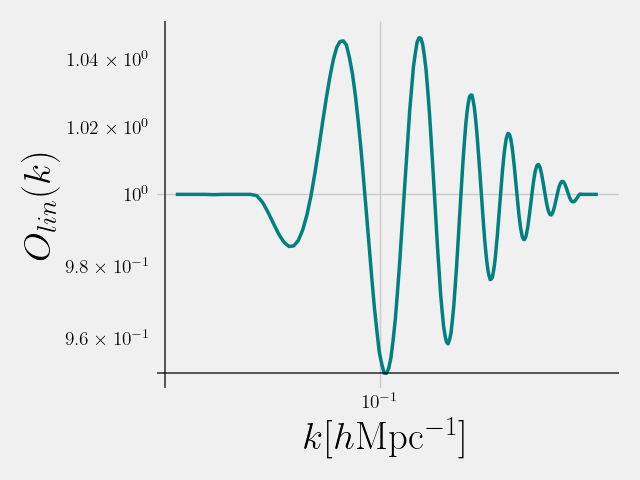
\includegraphics[width=0.3\textwidth]{../figs/Olin.png}}
	\caption{Graphic representation of the $P(k)$ (left panel), $P_{smooth}(k)$ (middle panel) and $O_{lin}(k)$ (right panel)for $\Omega_k = 0$.}
	\label{fig:PkOlPsm}
\end{figure}

Having the data, it is then necessary to have a model that explains it. The Cosmic Linear Anisotropy Solving System (CLASS) \cite{class} library allows the user to calculate the theoretical curve $P(k)$ should have for each cosmology. This software takes the corresponding cosmology as an input and returns the power spectrum seen in the leftmost panel of the figure~\ref{fig:PkOlPsm}. Note that this curve looks like a decreasing function which will be named $P_{\text{smooth}}(k)$, modulated by an oscilating curve, named $O_{\text{lin}}(k)$. These two functions are seen in the two leftmost panels of the figure~\ref{fig:PkOlPsm}, and verify 
\begin{align}
	P(k) = P_{\text{smooth}}(k) O_{\text{lin}}(k)
	\label{eq:pk-components}
\end{align}\\

To split the power spectrum $P(k)$ into these two functions, the routine \textit{remove\_bao} from the Montepython project~\cite{montepython} has been used. This routine takes as input the power spectrum $P(k)$ as an array of points. It then computes the geometrical curvature of the curve and interpolates in between the points at which the calculated curvature results in 0. The output of this function is the smoothed power spectrum $P_{\text{smooth}}(k)$. By the definition \eqref{eq:pk-components}, the pure BAO  $O_{\text{lin}}(k)$ are calculated through 
\begin{align}
	O_{\text{lin}}(k) = \frac{P(k)}{P_{\text{smooth}(k)}}
\end{align}

The relationship between the data and the model is done through the Bao and RSD Algorithm for Spectroscopy Surveys (BRASS)~\cite{brass}. This software allows for the calculation of the $\alpha$ parameters, as defined by \eqref{eq:alphas-def}. BRASS takes as input the calculated power spectrum (given by RUSTICO) for some  fiducial cosmology, and the theoretic power spectrum for some other fiducial cosmology. It will return among many other fit parameters, the $\alpha_\parallel$ and $\alpha_\perp$ parameters along with their standard deviations that will allow the calculation of the observables $D_H/r_s$ and $D_A /r_s$.\\

All of these calculations were done thanks to the clusters to which I was granted access to in Universidad de Córdoba. The hardware used (FQM-378) had the following specifications:
\begin{itemize}
	\item One node, named Pauli
	\item One CPU per node, \textit{Intel(R) Xeon(R) Silver 4210R CPU @ 2.40 GHz} with 40 threads
	\item 64Gb memory
	\item Operative System: Ubuntu 22.04.2 LTS, release 22.04, codename \textit{jammy}
\end{itemize}
